%% =====================================================================
%% NetPerturb -- Application Note for Bioinformatics Advances (OUP)
%%
%% FIRST DRAFT TEMPLATE. Everything marked \todo{...} (red) needs your input.
%%
%% Bioinformatics Advances limits for an Application Note (author guidelines):
%%   * up to 4 pages, including figures, tables and references
%%   * abstract: at most 200 words
%%   * at most 3 figures + tables COMBINED  (this draft: Fig 1, Fig 2, Table 1;
%%     the earlier van Galen figure moved to Supplementary Fig. S2)
%%   * at most 15 references                 (this draft cites 17 -- drop 2, e.g.
%%     Langfelder2008wgcna, Liberzon2015msigdb or Ewels2020nfcore)
%%   * at most 5 keywords
%%   * required statements: Data availability, Funding, Conflict of interest,
%%     Author contributions; ORCID for the submitting author; any AI/LLM use
%%     must be disclosed in the cover letter and Methods/Acknowledgements
%%
%% Build:  latexmk -pdf netperturb.tex
%% =====================================================================

\documentclass[unnumsec,webpdf,contemporary,large]{oup-authoring-template}
%\onecolumn % for one column layouts

\graphicspath{{../../Fig/}}
\newcommand{\societylogo}{}

% Draft helpers -- remove before submission
\newcommand{\todo}[1]{\textcolor{red}{[TODO: #1]}}
\newcommand{\np}{\textsc{NetPerturb}}
\newcommand{\param}[1]{\texttt{-{}-#1}}

% line numbers (often requested by reviewers)
%\usepackage[right]{lineno}

\begin{document}

\journaltitle{Bioinformatics Advances}
\DOI{DOI added during production}
\copyrightyear{2026}
\pubyear{2026}
\vol{XX}
\issue{x}
\access{Published: Date added during production}
\appnotes{Application Note}

\firstpage{1}

\subtitle{Gene Regulation and Systems Biology} % \todo: confirm journal subject section

\title[NetPerturb]{NetPerturb: a reproducible Nextflow pipeline for in silico perturbation of single-cell gene regulatory networks from a Seurat object}

\author[1,$\ast$]{Diego Marques-Coelho\ORCID{0000-0000-0000-0000}}
\author[1]{\todo{Second Author}}
\author[2]{\todo{Third Author}}

\address[1]{\orgdiv{\todo{Department}}, \orgname{\todo{Organization}}, \orgaddress{\street{\todo{Street}}, \postcode{\todo{Postcode}}, \state{\todo{State}}, \country{\todo{Country}}}}
\address[2]{\orgdiv{\todo{Department}}, \orgname{\todo{Organization}}, \orgaddress{\street{\todo{Street}}, \postcode{\todo{Postcode}}, \state{\todo{State}}, \country{\todo{Country}}}}

\corresp[$\ast$]{Corresponding author. \href{mailto:diegomscoelho@gmail.com}{diegomscoelho@gmail.com}}

\received{Date}{0}{Year}
\revised{Date}{0}{Year}
\accepted{Date}{0}{Year}

\editor{Associate Editor: Name}

%% ---------------------------------------------------------------------
%% Abstract: <= 200 words, structured, no citations.
%% ---------------------------------------------------------------------
\abstract{
\textbf{Motivation:} Predicting how a genetic or pharmacological perturbation affects each cell population in a single-cell RNA-seq (scRNA-seq) dataset is a common question, but in silico perturbation tools based on gene regulatory networks (GRNs) are hard to install, scale poorly to large atlases, and return results that are difficult to compare across methods and to share.\\
\textbf{Results:} We present NetPerturb, a Nextflow pipeline that starts from a processed Seurat object and a list of target genes and returns a single, self-contained HTML report. NetPerturb balances cell identities by downsampling, checks the targets before any network is built, and infers one GRN per identity with GENIE3, scRank or hdWGCNA. It then ranks identities by a target-perturbation score. In parallel, it can run a virtual knockout with scTenifoldKnk, including joint knockouts of several genes, followed by gene set enrichment of the genes the knockout affects. Every stochastic step is seeded from one parameter and every tool runs in a versioned container, so runs are reproducible on HPC and cloud. In four AML cohorts, target scores replicated (Spearman 0.88--0.92). Corrected for network size, IL3RA and KDM1A consistently favoured stem cells, mitotic kinases spared them, and blast markers KIT, FLT3 and CD33 favoured malignant identities.\\
\textbf{Availability and implementation:} NetPerturb is freely available under the \todo{MIT} licence at \url{https://github.com/MCBLab/NetPerturb}, with documentation, test profiles and container recipes. \todo{Zenodo DOI of the release.}\\
\textbf{Contact:} \href{mailto:diegomscoelho@gmail.com}{diegomscoelho@gmail.com}\\
\textbf{Supplementary information:} Supplementary data are available at \textit{Bioinformatics Advances} online.}

\keywords{single-cell RNA-seq, gene regulatory network, in silico perturbation, virtual knockout, Nextflow}

\maketitle

%% =====================================================================
\section{Introduction}
%% =====================================================================

Single-cell RNA-seq (scRNA-seq) resolves tissues into cell identities (cell types, clones, or treatment states), and the next question is usually which of those identities depend on a given gene or drug target. Pooled CRISPR screens with single-cell readout answer this experimentally \citep{Dixit2016perturbseq}, but they are costly and cannot be applied to archived or clinical samples. Computational alternatives therefore perturb a gene regulatory network (GRN) inferred from unperturbed cells and read the effect off the network: CellOracle simulates shifts in cell identity \citep{Kamimoto2023celloracle}, scRank ranks cell types by how much a drug target reshapes their network \citep{Li2024scrank}, and scTenifoldKnk performs a virtual knockout and reports the genes whose regulatory context changes \citep{Osorio2022sctenifoldknk}.

In practice, using these methods on a new dataset takes considerable engineering work. Each method expects its own input format and gene universe, and memory grows quickly with the number of cells and genes. Targets that are not expressed in some identities can end a run late in the analysis. Results from different network inference methods are rarely placed side by side, and many steps are stochastic, so the numbers are hard to reproduce. \todo{Add 1--2 sentences on the specific gap your lab hit.}

NetPerturb addresses this with a single Nextflow \citep{DiTommaso2017nextflow} workflow, organised following nf-core practice \citep{Ewels2020nfcore}. Its input is the object most analysts already have, a processed Seurat object \citep{Hao2023seurat}. It parallelises network inference and scoring across identities and targets, and it gathers every result, together with the quality control and provenance needed to interpret it, into one portable report.

%% =====================================================================
\section{Implementation}
%% =====================================================================

\begin{figure*}[!t]%
\centering
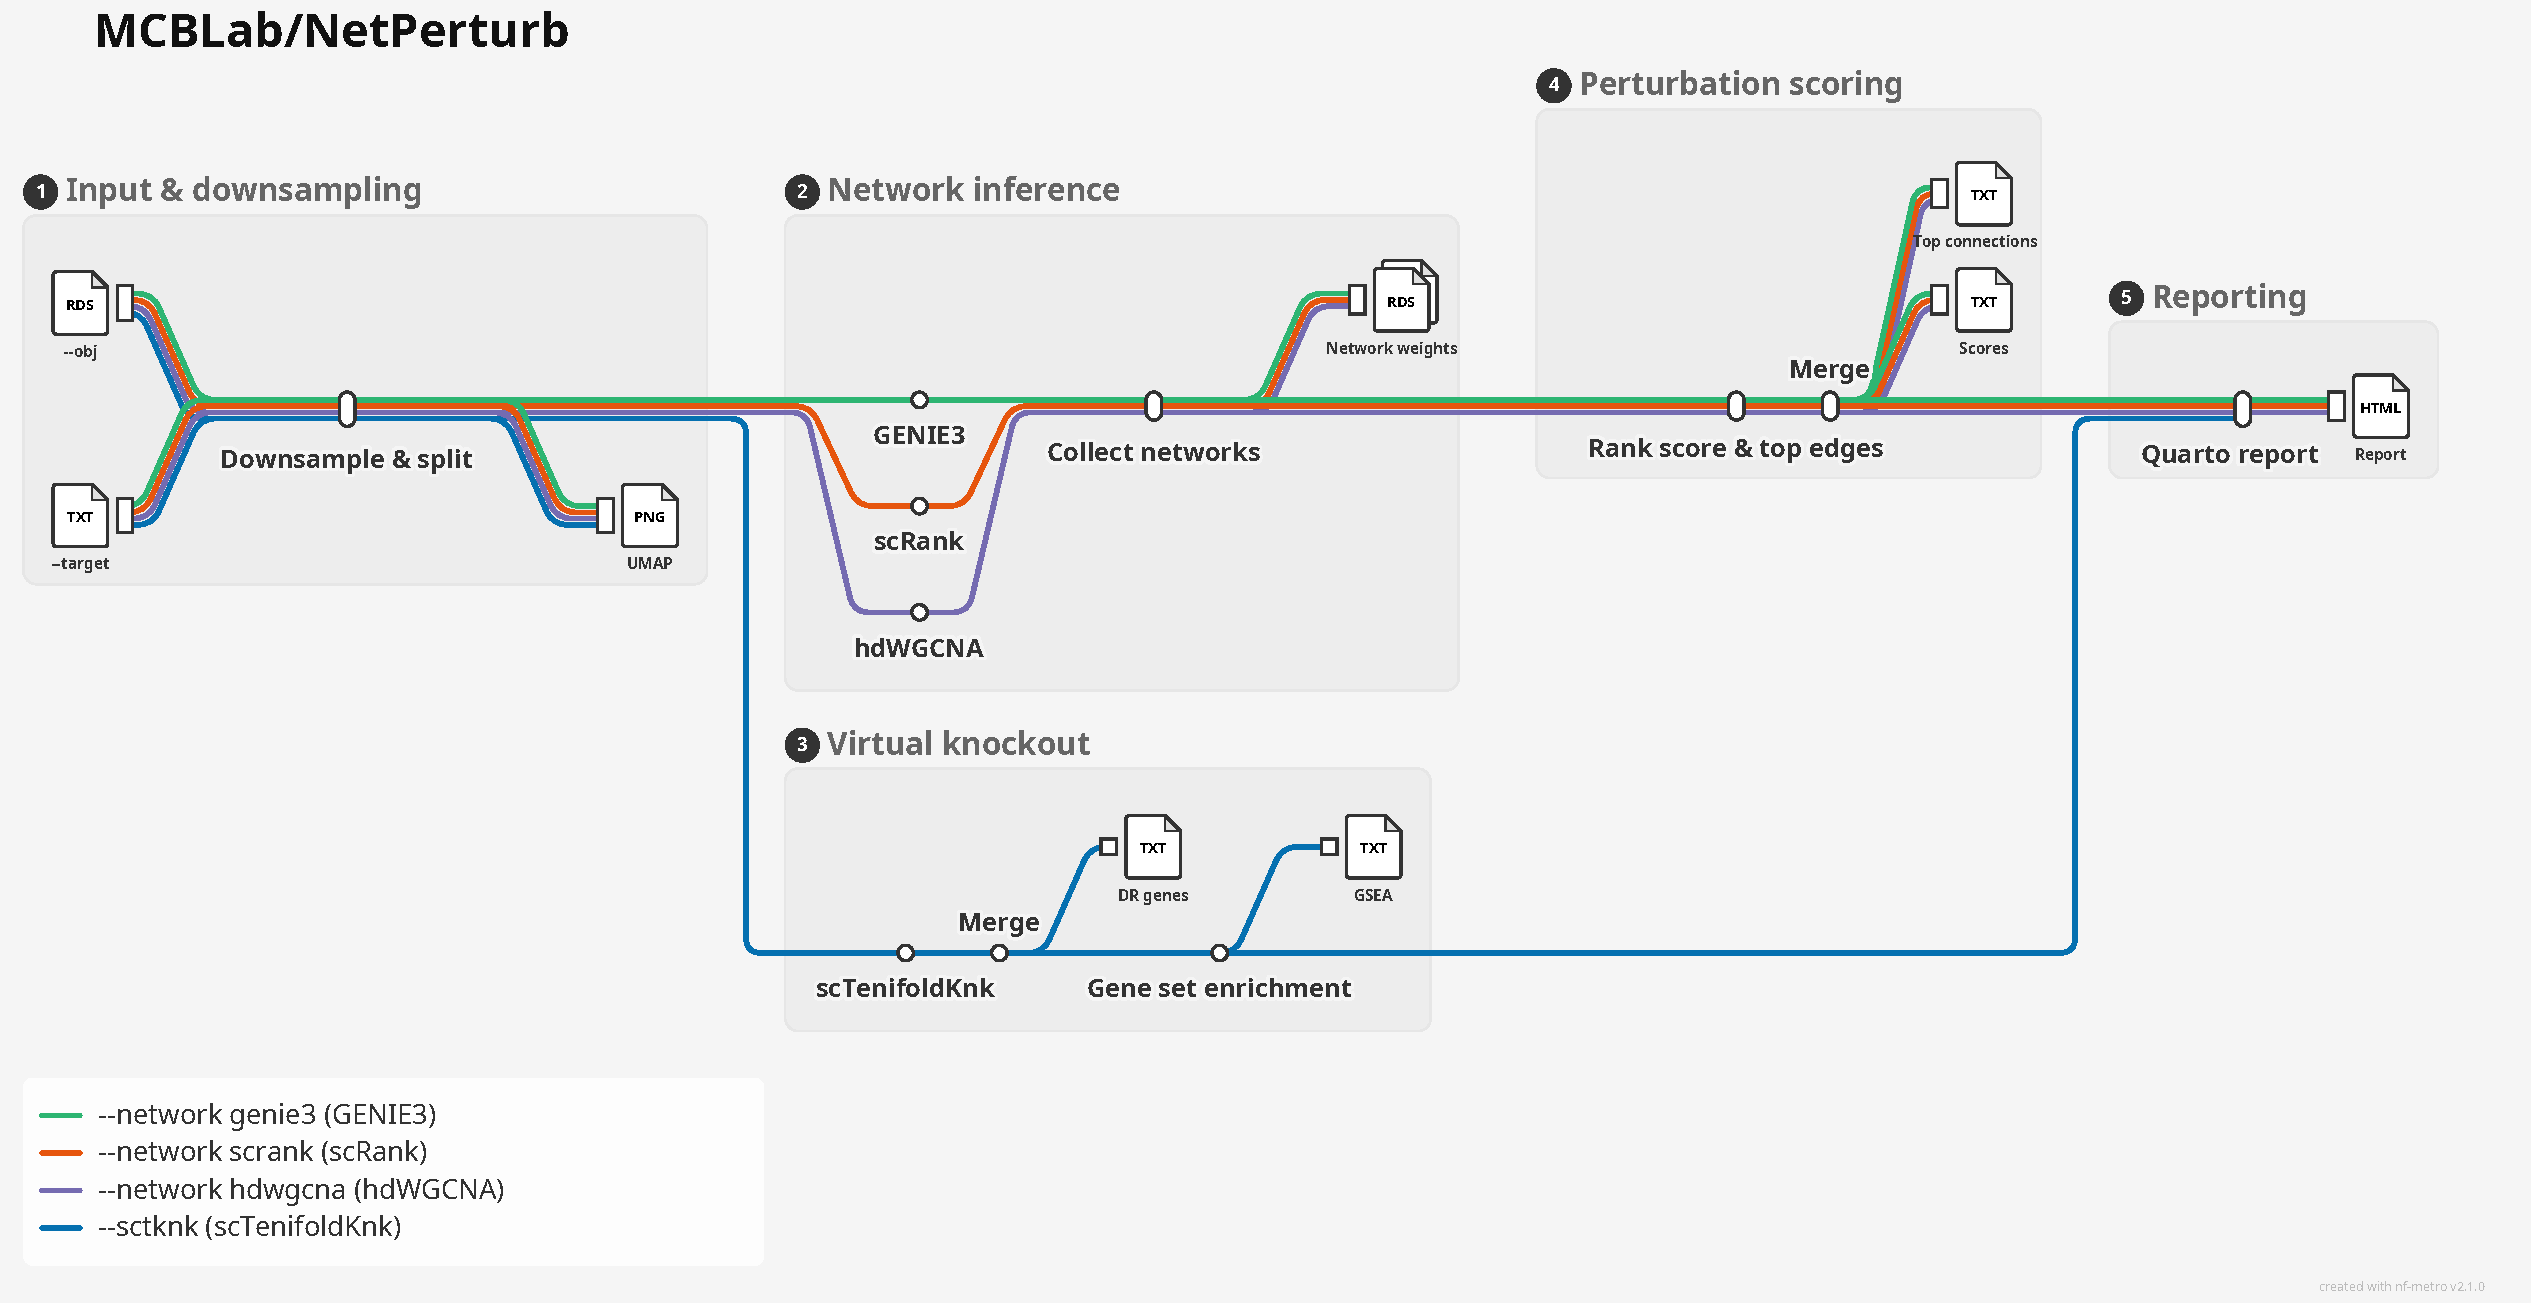
\includegraphics[width=\textwidth]{fig1_metro.pdf}
\caption{\textbf{Overview of NetPerturb.} A processed Seurat object and a list of target genes enter \texttt{DOWNSAMPLE}, which balances cell identities and checks the targets. The rank-score track (warm lines; one of GENIE3, scRank or hdWGCNA, chosen with \param{network}) infers one GRN per identity and scores every identity $\times$ target pair. The knockout track (blue; \param{sctknk}) builds one wild-type scTenifoldKnk network per identity and runs one virtual knockout per identity $\times$ target, optionally followed by fgsea. Both tracks converge on a single self-contained HTML report.}\label{fig:overview}
\figalttext[Metro-map diagram of the NetPerturb pipeline]{Metro-style diagram in which coloured lines represent the three alternative network inference methods and the parallel scTenifoldKnk knockout track, running from input through downsampling, network inference, scoring, merging and enrichment to the HTML report.}%
\end{figure*}

\subsection{Input and pre-processing}

NetPerturb requires four inputs: a Seurat object (\param{obj}), the metadata column defining cell identities (\param{column}), the species, and a text file of targets (\param{target}), one per line. Genes joined by a semicolon (e.g.\ \texttt{CDK8;CDK19}) are treated as a single combined perturbation. The \texttt{DOWNSAMPLE} step randomly keeps at most \param{n\_cells} cells per identity, so that every identity contributes a comparable number of cells, and drops identities that end up with fewer than \param{min\_cells} cells. It also builds a shared gene universe from the highly variable genes, transcription factors, drug targets and the requested targets. Each target is checked against the retained cells before any network is built. Genes that are absent from the object or have no counts are removed and recorded, a combined target keeps whichever of its genes pass, and the run stops only when no target passes. Problems that would otherwise end a run hours later are therefore caught at the start and listed in the report.

\subsection{Rank-score track}

For each identity, NetPerturb infers a GRN with one of three interchangeable methods (Table~\ref{tab:methods}). GENIE3 \citep{HuynhThu2010genie3} and scRank's own network builder \citep{Li2024scrank} are used as published. hdWGCNA \citep{Morabito2023hdwgcna}, which builds on WGCNA \citep{Langfelder2008wgcna}, produces an unsigned co-expression network on metacells, so NetPerturb adapts its topological overlap matrix to the input scRank expects in four steps. It restores the sign of each edge from the correlation between the two genes, pads every identity to the same gene set, removes edges below the \param{cut\_ratio} quantile of absolute weight, and rescales the weights to $[-1,1]$. Each identity $\times$ target pair is then scored with scRank, which compares each network before and after removing the target's edges and returns a perturbation score in either antagonist or agonist mode. The strongest \param{top\_connections} edges of each target are also exported. Networks and scores are computed as separate parallel tasks and merged into one table afterwards.

\begin{table}[!t]
\begin{center}
\begin{minipage}{\columnwidth}
\caption{Network inference methods available in NetPerturb.\label{tab:methods}}%
\small\begin{tabular}{@{}llll@{}}
\toprule
Method & Network & Output & Track \\
\midrule
GENIE3      & Tree-based regression  & Directed weights       & Rank score \\
scRank      & scRank builder   & Directed weights       & Rank score \\
hdWGCNA     & Metacell TOM + sign    & Signed, sparsified     & Rank score \\
scTenifoldKnk & PCR + tensor denoising & WT vs.\ KO manifold  & Knockout \\
\botrule
\end{tabular}
\begin{tablenotes}%
\item TOM, topological overlap matrix; PCR, principal component regression; WT, wild type; KO, knockout.
\end{tablenotes}
\end{minipage}
\end{center}
\end{table}

\subsection{Virtual knockout track}

When \param{sctknk} is set, a scTenifoldKnk track \citep{Osorio2022sctenifoldknk} runs alongside the rank-score track, or on its own. The expensive wild-type network does not depend on the target, so NetPerturb builds it once per identity (\texttt{SCTENIFOLDKNK\_BUILD}). Each identity $\times$ target knockout then runs as a separate task on that stored network (\texttt{SCTENIFOLDKNK\_KO}). With a single build per identity, one wild-type network can serve any number of knockouts, and the knockout of a combined target can zero the edges of all its genes at once, which the original single-gene interface does not allow. Differential regulation uses the statistic of scTenifoldKnk v1.0.3, which leaves the knocked-out genes out of the reference mean. Because the genes an alignment moves most are the network's hubs whatever the target, each gene is also tested against the same knockout run for random genes of the network (\param{sctknk\_null}), a target with no outgoing edge is skipped as a no-op, and the rank of the tensor decomposition is a parameter (\param{sctknk\_td\_k}). If a GMT file is supplied, genes are ranked by $\log_2$FC and tested with fgsea \citep{Korotkevich2016fgsea} against, for example, MSigDB collections \citep{Liberzon2015msigdb}. Gene sets are read from local files, so the step also runs on compute nodes without internet access.

\subsection{Report}

The \texttt{REPORT} step renders a single self-contained Quarto HTML file (\todo{Supplementary Fig.~S1: report screenshots}). The report contains:
(i) an overview recording the network method, the targets removed by quality control, the number of cells and genes available to each identity's network, and a UMAP of the retained cells;
(ii) a heatmap of target expression per identity, so that a low score can be checked against a target that is barely expressed;
(iii) a searchable table and a heatmap of perturbation scores;
(iv) interactive knockout networks and a table of differentially regulated genes;
(v) an enrichment dot plot and table; and
(vi) provenance, with the command line, software versions, parameters and the running time of each step taken from the Nextflow trace.

\subsection{Reproducibility and deployment}

Every tool runs in a versioned Singularity/Docker container \citep{Kurtzer2017singularity}, so no R dependencies need to be installed. A single \param{seed} parameter sets the random seed of every step that uses one: downsampling, GENIE3 (via doRNG), hdWGCNA metacells, scTenifoldKnk and fgsea. scRank's network builder is the one exception, because it sets its own seed internally. Memory and CPU requests are defined per process and can be adjusted in a configuration profile. The pipeline is tested with nf-test at the module and workflow level, and it provides small and dataset-scale test profiles (\texttt{-profile test}).

%% =====================================================================
\section{Results}
%% =====================================================================
%% Numbers below are produced by analysis/fig2_zeng.R -> analysis/zeng_cohort_stats.txt
%% (per-target table: analysis/zeng2025/target_effects.tsv).
%% Earlier single-cohort run, now Supplementary Fig. S2 (Fig/fig2_vangalen_genie3.pdf):
%% analysis/fig2_vangalen.R genie3 -> analysis/vangalen_stats_genie3.txt

We benchmarked the rank-score track on four acute myeloid leukaemia (AML) cohorts, asking whether its results replicate between cohorts and how the targets of AML drugs act across the haematopoietic hierarchy. The knockout track was not part of this benchmark.

\begin{figure*}[!t]%
\centering
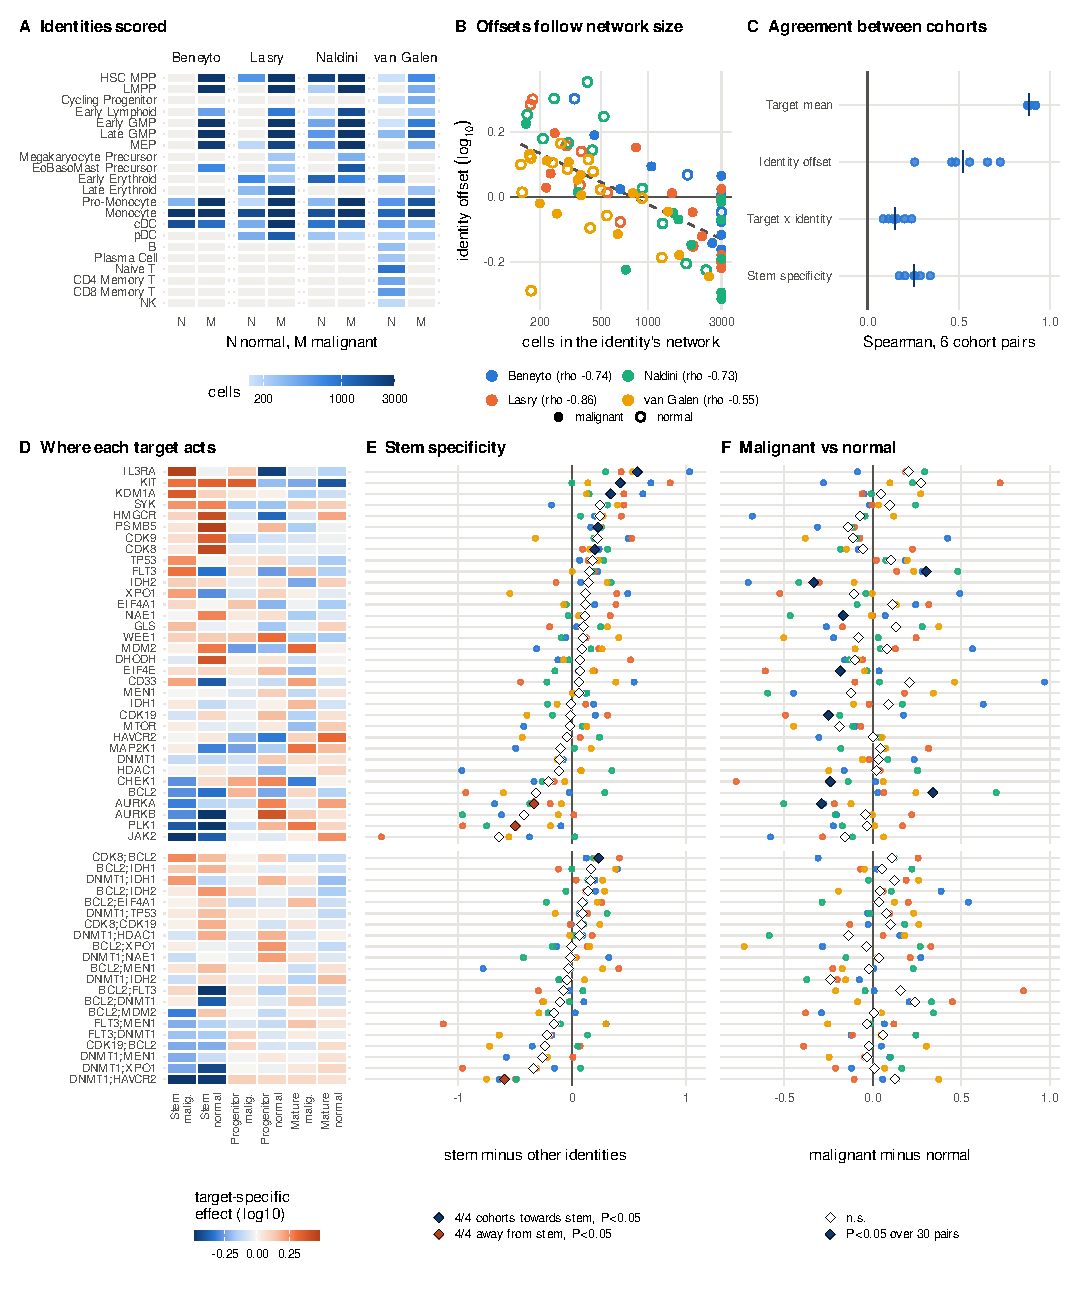
\includegraphics[width=\textwidth]{fig2_zeng_cohorts.pdf}
\caption{\textbf{Multi-cohort benchmark of the rank-score track on AML} (four cohorts of the \citet{Zeng2025bonemarrowmap} atlas; GENIE3 networks, antagonist mode, 55 targets). (A) Identities scored per cohort, normal (N) and malignant (M), coloured by the number of cells the network was built from; grey, not scored. (B) Identity-wide offset, from a decomposition of $\log_{10}$ scores into target and identity effects, against the identity's number of cells; filled, malignant. (C) Spearman correlation over the six pairs of cohorts for the target mean, the identity offset and the target-specific effect (12 identities scored in every cohort), and for stem specificity (E); bars, medians. (D) Target-specific effect (residual of the $\log_{10}$ score once target and identity effects are removed), averaged over the identities of each compartment and over cohorts; stem, HSC/MPP and LMPP. (E) Stem specificity: target-specific effect in stem identities minus that in all other identities, per cohort (dots) and averaged (diamonds); filled diamonds, same sign in all four cohorts and permutation $P<0.05$. (F) Malignant minus matched normal identity, per cohort (dots) and over all 30 pairs (diamonds; filled, signed-rank $P<0.05$). In D--F, targets are ordered by stem specificity, single genes above joint targets.}\label{fig:bench}
\figalttext[Six-panel multi-cohort benchmark figure on AML data]{Panel A is a tile chart of the identities scored in four cohorts, split into normal and malignant. Panel B is a scatter plot in which identity offsets fall as the number of cells rises, in every cohort. Panel C shows cohort-pair correlations near 0.9 for target means and below 0.35 for target-specific effects and stem specificity. Panels D to F share a target axis: a heatmap of target-specific effects by compartment, and dot plots of stem specificity and of malignant-minus-normal differences, with IL3RA, KIT and KDM1A at the stem end and the mitotic kinases at the other.}%
\end{figure*}

\paragraph{Data and runs.} \citet{Zeng2025bonemarrowmap} mapped the cells of 21 published AML scRNA-seq studies onto a reference of normal haematopoiesis. We took four of these cohorts, those of Beneyto-Calabuig, Lasry, Naldini and \citet{vanGalen2019aml}, and called every cell malignant or normal with scMalignantFinder \citep{Yu2025scmalignantfinder}. Its pre-trained pan-cancer model did not separate AML blasts from normal cells (58\% agreement with van Galen's labels), so we retrained it on the curated labels of the other three cohorts. On the held-out van Galen cohort it then agreed with the original labels for 81\% of cells (AUC 0.88); for the other three cohorts the call is in-sample. \todo{Confirm that the final calls used this retrained model (3 cohorts, logistic regression).} Each identity combines the atlas's broad cell type with this call, a malignant identity carrying the suffix \emph{-like} (e.g.\ HSC\_MPP-like). We ran NetPerturb on each cohort with GENIE3, antagonist mode, \param{n\_cells}~3,000, \param{min\_cells}~150 and 55 targets of drugs used or trialled in AML (BCL2, FLT3, IDH1, IDH2, MEN1, DNMT1, KIT, CD33, IL3RA and others; 34 single genes and 21 pairs). NetPerturb kept 13--27 identities per cohort, 86 in all (111,592 cells; Fig.~\ref{fig:bench}A), and dropped another 54 below \param{min\_cells} automatically. Every target passed quality control, and only 13 of the 4,730 identity $\times$ target pairs had no score.

\paragraph{Target-level scores replicate across cohorts.} Within a cohort, the target explained 38--54\% of the variance of $\log_{10}$ scores and the identity 3--8\%. A target's mean score agreed closely between cohorts (pairwise Spearman $\rho$ 0.88--0.92; Fig.~\ref{fig:bench}C), and with an earlier run on van Galen's original labels and an older pipeline version ($\rho=0.84$; \todo{Supplementary Fig.~S2}). The target-specific part of a single identity $\times$ target score, the residual left once the target and identity effects are removed, replicated far less ($\rho$ 0.09--0.24 over the 12 identities scored in every cohort). We therefore draw conclusions only from effects aggregated over identities and cohorts.

\paragraph{Identity offsets follow network size.} Identity-wide offsets spanned 0.45--0.67 $\log_{10}$ per cohort, and they fell as the number of cells behind the identity's network rose ($\rho$ $-0.55$ to $-0.86$; Fig.~\ref{fig:bench}B). This matters in AML, where malignant identities usually reach the \param{n\_cells} cap and their normal counterparts do not (median 1,917 against 407 cells). Without adjustment, malignant identities scored 0.13 $\log_{10}$ below normal ones ($P=10^{-4}$). With the number of cells in the model ($-0.26$ $\log_{10}$ per tenfold more cells, $P=10^{-12}$), the difference vanished ($-0.03$, $P=0.32$), and stem identities (HSC/MPP and LMPP) scored, if anything, below progenitor and mature ones (by 0.08 and 0.07). Stem cells were therefore not more affected across the board. Offsets report how large an identity's network is, not how vulnerable its cells are, so the comparisons below use the target-specific part of each score.

\paragraph{Targets that consistently act on stem cells.} For each target and cohort, we took the target-specific effect averaged over stem identities minus that averaged over all others (Fig.~\ref{fig:bench}E). The mean over cohorts was tested against 10,000 permutations of identity labels within each cohort. Six targets acted more on stem identities in all four cohorts with $P<0.05$: IL3RA ($+0.57$ $\log_{10}$, FDR 0.04), KIT ($+0.42$), KDM1A ($+0.34$, FDR 0.04), PSMB5, CDK8 and the joint target CDK8;BCL2. HMGCR, TP53, FLT3 and DNMT1;IDH1 were positive in all four cohorts without reaching $P<0.05$. The ranking held when stem was restricted to HSC/MPP ($\rho=0.89$) and when within-identity ranks replaced residuals ($\rho=0.94$). These targets split by the stem cells they act on (Fig.~\ref{fig:bench}D). IL3RA (CD123), a marker of leukaemic stem cells, acted on malignant stem identities ($+0.68$) and not on normal ones ($-0.02$), and it was higher in malignant than in normal stem cells in each of the three cohorts that have both. FLT3 behaved the same way ($+0.31$ against $-0.34$), and KDM1A (LSD1) did to a lesser degree ($+0.37$ against $+0.11$). PSMB5, CDK8 and HMGCR instead acted mostly on normal HSC/MPP ($+0.43$ to $+0.53$, against $+0.04$ to $+0.11$ in malignant stem cells), and KIT acted on both. These profiles predict haematopoietic toxicity rather than a selective effect on leukaemic stem cells. At the other end, the mitotic kinases AURKA and PLK1 acted less on stem identities in all four cohorts ($P<0.05$), as did CHEK1 ($P=0.10$), in line with stem-cell quiescence. The joint target DNMT1;HAVCR2 had the strongest effect in this direction ($-0.59$, FDR 0.005).

\paragraph{Malignant against normal identities.} Across the 30 matched pairs of a malignant identity and its normal counterpart (Fig.~\ref{fig:bench}F), the blast markers KIT, FLT3 and CD33, singled out in the earlier van Galen run, gained more than the other targets in 23 pairs (median $+0.27$ $\log_{10}$, signed-rank $P=1.5\times10^{-4}$). Individually, FLT3 ($+0.30$, 73\% of pairs, $P=0.003$) and BCL2 ($+0.34$, 70\%, $P=0.02$) led, and both, with IL3RA, were higher in malignant than in normal stem cells in every cohort that has both. BCL2, the target of venetoclax, was nonetheless not stem-specific relative to the other identities ($-0.32$). AURKA ($-0.29$, $P=0.001$) and IDH2 ($-0.33$, $P=0.004$) were lower in malignant identities. IDH1/2 inhibitors act on a mutant enzyme whose activity an expression network cannot see, so these targets are not expected to follow malignancy. No single target passed FDR 0.05 in this comparison (lowest 0.06).

\paragraph{Earlier single-cohort run.} A run on van Galen's own malignant/normal labels and 19 identities (\todo{Supplementary Fig.~S2}) gave the same picture. Malignant progenitors exceeded their normal counterparts most for KIT, FLT3 and CD33 (median 0.90 $\log_{10}$ over the three progenitor pairs, against 0.13 for the other targets, $P=0.006$), on top of identity offsets of up to 0.47 $\log_{10}$. Joint targets did not reproduce either member's profile (median Spearman $\rho$ 0.02 with the stronger member): a joint target is perturbed as one knockout of both genes' edges, and what the network then loses is not what it loses for either gene alone. \todo{That run predates the mito/ribo removal and the Data quality section (25 Sep); the four-cohort runs above use the current pipeline. Re-run or drop Supplementary Fig.~S2 before submission.}

\paragraph{Cost.} A cohort took 15--43\,h of compute, almost all of it GENIE3: on average 0.4--2.7\,h per identity, and up to 4.7\,h for an identity at the 3,000-cell cap. Scoring then took 4--6\,min per target. Every identity and every target is its own task, so on a cluster a cohort finishes in about the time of its longest task, under 5\,h.


%% =====================================================================
\section{Conclusion}
%% =====================================================================

NetPerturb takes an analyst from a Seurat object to a shareable report on GRN-based in silico perturbation with a single command. It runs several network inference methods and a virtual knockout under one interface, and its seeding, containers and provenance make each result reproducible. The four-cohort benchmark also shows how these scores should be read. Target-level results replicated between cohorts, but single identity $\times$ target scores did not, so conclusions should rest on effects aggregated over identities and, where possible, over cohorts. Scores carry an identity-wide offset that tracks how many cells an identity's network was built from. Identities should therefore be compared through the target-specific part of the score, or against control targets from the same run, and not through raw scores. Scores follow how strongly an identity's network relies on the target, which tracks the target's expression there rather than a drug's clinical sensitivity. They are comparable only within one inference method. Read this way, the scores placed IL3RA, KDM1A and FLT3 on malignant stem cells and PSMB5, CDK8 and HMGCR on normal ones, and showed mitotic kinases sparing stem cells in all four cohorts. The knockout track was not evaluated here; it ships with a random-knockout null model for the same reason the offsets above exist. \todo{Future work: e.g.\ downsampling every identity to the same number of cells, which would remove most of the offset; built-in control targets and a per-identity null; detection filter on targets; AnnData input; nf-core submission.}

%% =====================================================================
%% Back matter -- all required by Bioinformatics Advances
%% =====================================================================

\section{Acknowledgements}
\todo{Acknowledgements.} \todo{AI disclosure: the guidelines require disclosing any AI/LLM use (e.g.\ assistance with code or drafting) here or in Methods, as well as in the cover letter.}

\section{Author contributions}
\todo{CRediT roles, e.g.\ D.M.-C.: Conceptualization, Software, Writing -- original draft. \ldots}

\section{Conflict of interest}
None declared.

\section{Funding}
\todo{Funding agencies and grant numbers.}

\section{Data availability}
The source code, container recipes and test data definitions are available at \url{https://github.com/MCBLab/NetPerturb} (release \todo{vX.Y.Z}, archived at Zenodo \todo{DOI}). The multi-cohort benchmark uses the processed objects of \citet{Zeng2025bonemarrowmap} (Zenodo, \href{https://doi.org/10.5281/zenodo.18528442}{doi:10.5281/zenodo.18528442}) for the cohorts of Beneyto-Calabuig, Lasry, Naldini and \citet{vanGalen2019aml} (GEO accession GSE116256), with malignant/normal calls from scMalignantFinder. The re-annotated Seurat objects, the retrained classifier and the benchmark outputs are available at \todo{Zenodo DOI}.

%% ---------------------------------------------------------------------
%% References: numbers are capped at 15 for an Application Note.
%% references/references.bib also holds uncited entries (GEARS, van Galen, Ocasio)
%% that are not cited yet, in case you want to swap them in.
%% ---------------------------------------------------------------------
\bibliographystyle{oup-abbrvnat}
\bibliography{../../references/references}

\end{document}
